When selecting sensors for this project, the team had to select PM2.5 and CO$_2$ sensors that were energy efficient, relatively accurate for our setting, and fit within a budget of \$3,000 for all 10 possible nodes. \\
\\
When selecting the CO$_2$ sensor, the team considered selecting a true CO$_2$ sensor like the SCD30 which would produce very accurate readings yet was more expensive than an ECO2 (estimated CO$_2$) sensor which would prove to be less accurate due to its nature of estimating CO$_2$ based on ethanol and H$_2$ levels in the air. Our team ultimately chose to go with the SGP30 (equivalent CO$_2$) sensor as we are merely sensing elevated levels of carbon dioxide and therefore do not need to get incredibly precise readings. Anything over 1,000 PPM would simply be very high and might constitute an evacuation of room or need for more airflow. \\
\\
\begin{table}[h]
\centering
\begin{tabular}{|l|l|l|}
\hline
Sensor             & SGP 30      & SCD 30                   \\ \hline
Type               & eCO$_2$      & CO$_2$                     \\ \hline
Additional sensors & VOC         & temperature and humidity \\ \hline
Range              & 400-60,000 PPM & 400-10,000 PPM              \\ \hline
Accuracy           & $\pm$15\%      & $\pm$30 PPM +3\%              \\ \hline
Price              & \$17.50      & \$58.95                   \\ \hline
\end{tabular}
\caption{CO$_2$ Sensor Finalists}
\label{tab:CO_2 Sensor Finalists}
\end{table}
\\
\subsection{PM2.5 Sensor}
For the PM2.5 sensor, the team decided to go with the SPS30 as it was the least power hungry among our options at the time. It was also the most readily available, and was sourced from Sensirion like the SGP30 which would cut costs if this product were to be mass produced. The PM2.5 Sensor Finalists table below shows the specific trade offs our team considered when selecting this sensor.\\
\\
\begin{table}[h]
\centering
\resizebox{\textwidth}{!}{%
\begin{tabular}{|l|p{4cm}|p{4cm}|p{4cm}|}
\hline
Sensor                      & PMS5003                                                                & PAS-IN-01                                & SPS30                                    \\ \hline
Range (concentration)       & 0-500 ug/m\textasciicircum{}3            & 0-1500 ug/m\textasciicircum{}3           & 0-1000 ug/m\textasciicircum{}3           \\ \hline
Accuracy                    & ±10\% or ±10 ug/m3, whichever is greater &  ±10\% or ±10 ug/m3, whichever is greater & ±10\% or ±10 ug/m3, whichever is greater \\ \hline
Power Consumption (on)      & $\sim$500mW                                                        & $\sim$350mW                              & $\sim$275mW                              \\ \hline
Price                       & \$39.95                                                                & \$19                                     & \$49.53                                  \\ \hline
Accurate data & 30 seconds                                                           & 15 seconds                               & 10 seconds                               \\ \hline
\end{tabular}
}
\caption{PM2.5 Sensor Finalists}
\label{tab:PM2.5 Sensor Finalists}
\end{table}
\subsection{Anemometer}
When selecting an anemometer, we originally preferred the concept of designing and building an ultrasonic anemometer as it was significantly more energy efficient than hot wire anemometer options. Due to issues with building a custom sensor as well as difficulties with procuring parts in a speedy manner, we decided to pivot to a hot wire anemometer. This selection produced a drastic detriment to our anticipated battery life. We originally calculated that we could complete the project with just 1 battery, however we needed to add 3 more batteries to achieve the same battery life of a year with the substitution of a hot wire anemometer. To accommodate for the increased temperature, we also had to give the part extra space and keep it as far away from our other sensors as possible. We suggest future builds expand upon our ultrasonic anemometer research, implementation and documentation in an attempt to prevent the use of hot wire anemometers in this setting. \\
% Please add the following required packages to your document preamble:
% \usepackage{graphicx}
\begin{table}[h]
\centering
\resizebox{\textwidth}{!}{%
\begin{tabular}{|l|l|l|}
\hline
Sensor                 & Custom Ultrasonic Anemometer & PAS-OUT-01Wind Sensor Rev. C                                 \\ \hline
Range                  & Unknown and size dependent   & 0-60 MPH                                                     \\ \hline
Power consumption (on) & $\sim$14.52mW                & $\sim$150mW                                                  \\ \hline
Accuracy               & Unknown and size dependent   & Can detect "small puff of air at a distance of 18-24 inches" \\ \hline
Price                  & \$7.90                       & \$21.95                                                      \\ \hline
Relative size          & $\sim$25-36 cm apart         & .68" x 1.59" x .25"                                          \\ \hline
\end{tabular}%
}
\caption{Anemometer Sensor Finalists}
\label{tab:Anemometer Sensor Finalists}
\end{table}
\\
\begin{figure}[H]
    \centering
    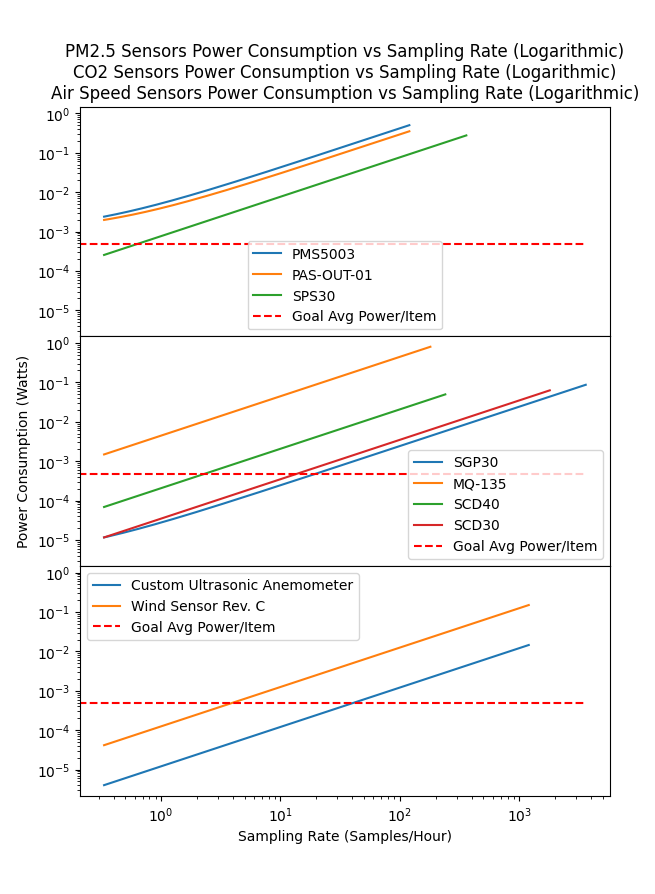
\includegraphics[width=0.8\textwidth]{Pictures/image (1).png}
    \caption[Power consumption measurements with sensor options]{Power consumption measurements with sensor options} 
    \label{fig:part1commrin}
\end{figure}
In Figure 2, the team created a python script to calculate the power consumption based on listed values from the specification sheets of the sensors. The python script can be found under the power testing folder in the documentation folder. The python script is titled \texttt{powerEstimation.py}. The link for the team Github page can be found in the project resources section. The red line shows the sampling rate needed to hit 1 year of battery life based on the estimates. \\
\\
%Below are some links to the sites we used when determining the ideal location for
%the sensors Sensor installation. FORMAT LINK
\\
\subsection{Enclosure}
When deciding on our enclosure. We wanted to minimize our SWaP-C, which stands size, weight, power, and cost. For our first iteration, we built a system utilizing Portland State University’s 3D printing. The 3D printer at the time only offered SLA. The helpers at the Electronics Prototyping Lab (EPL) recommended we switch to laser cutting acrylic as it is much cheaper, faster, and is clear. To cut the enclosure, we used MakerCase (https://www.makercase.com/\#/) as recommended by the EPL. The laser cutter utilized at the time of project was the QD-1390. \\
\\
\begin{figure}[H]
    \centering
    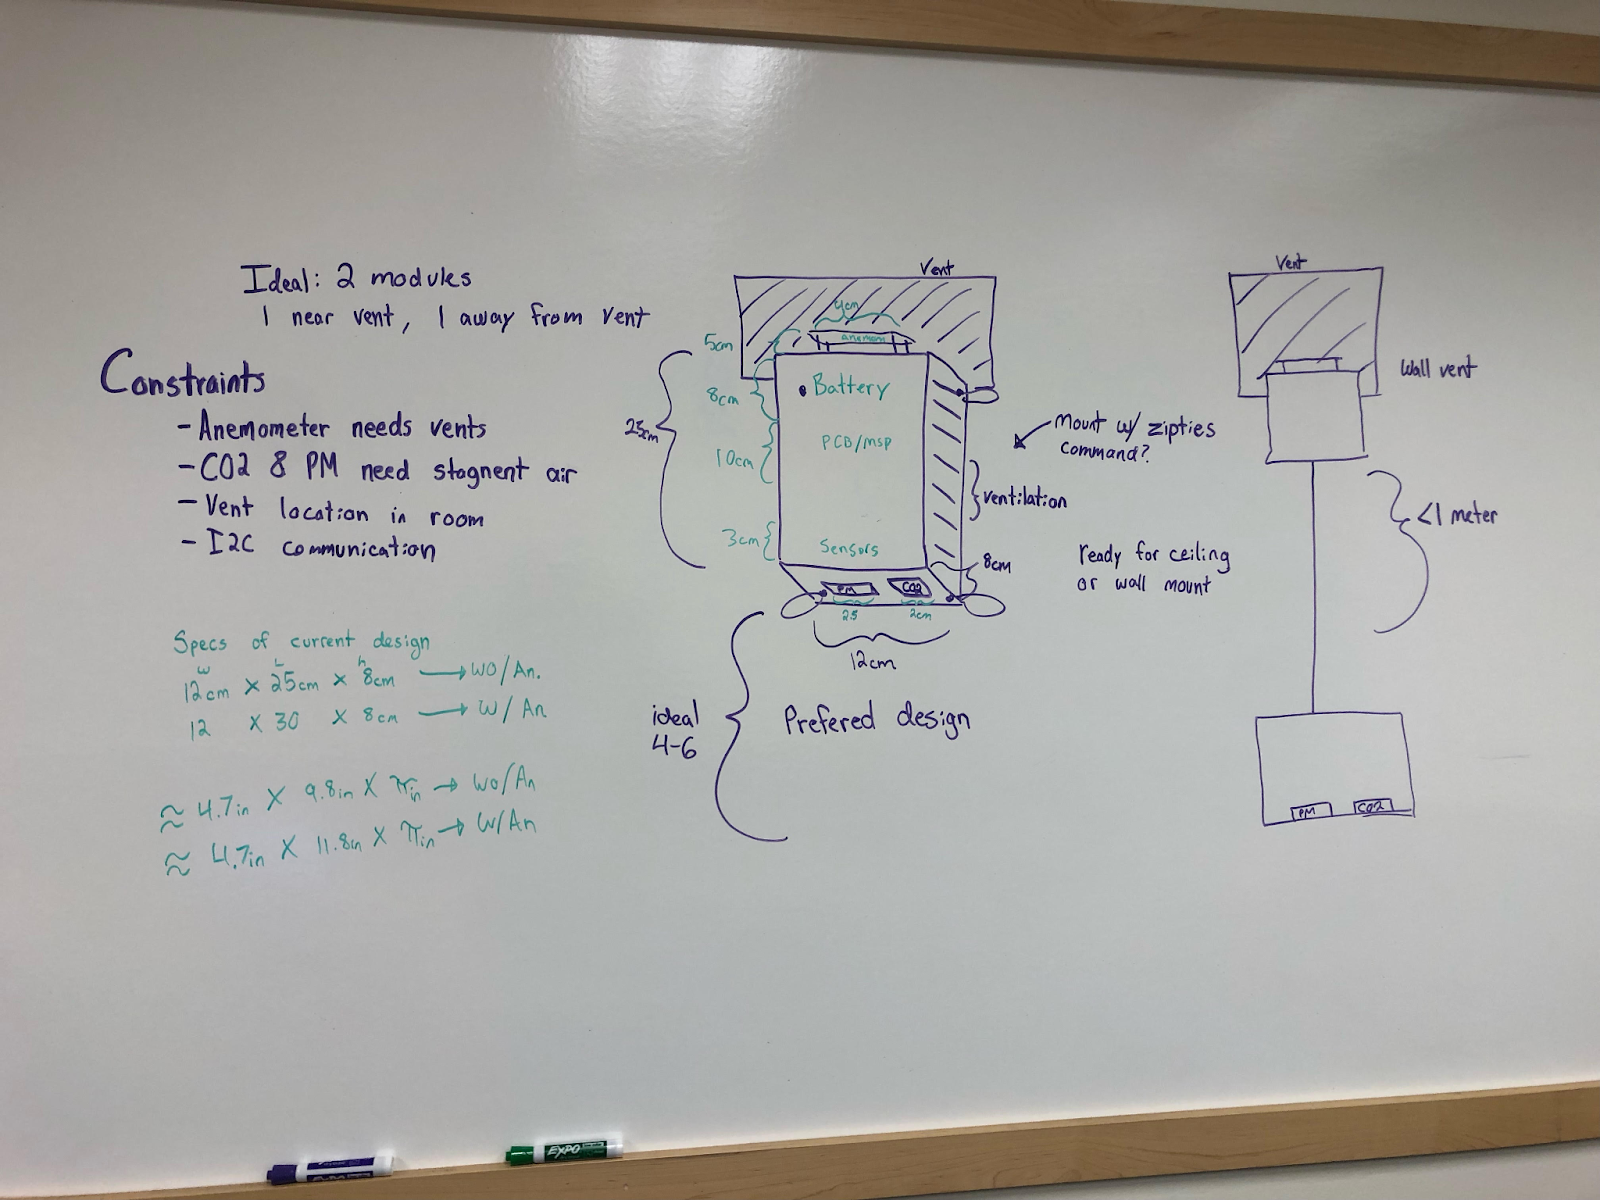
\includegraphics[width=0.8\textwidth]{Pictures/image (2).png}
    \caption[Original concepts for enclosure]{Original concepts for enclosure} 
    \label{fig:part1commrin}
\end{figure}
When designing the enclosure, we originally came up with the two ideas shown above. The rightmost diagram represented 2 enclosures separated by an I2C cable. This would allow us to get accurate readings for CO$_2$ and PM2.5 in the bottom enclosure, and accurate anemometer readings in the above enclosure. Having two nodes seperated by an I2C cable would allow for the anemometer to be placed near a vent while the CO$_2$ and PM2.5 sensors could be placed in the desired range for accurate readings. This design proved to be infeasible because we were limited by the maximum 1 meter length for an I2C cable. We switched to the design on the left focusing on increased ventilation and allowing for proper separation of parts to ensure no damage is caused by the batteries. We also aligned the sensors to face downwards while the anemometer could face sideways towards the vent. Final dimensions came out to be 
12 x 25 x 8 cm without an anemometer and
12 x 30 x 8 cm with an anemometer. This design requires several modules to be placed in one room, with an anemometer node being placed in front of an air vent while a second node without an anemometer could be placed in a stagnant area of the room. This accounts for both air entering the room as well as an accurate measurement of the air quality in the room. The non anemometer node should ideally be placed four to six feet above the ground as according the Environmental Protection Agency (EPA) for the most accurate CO$_2$ and PM2.5 readings

\subsection{System Design}
At the highest level view our system design started very simple. We have our microcontroller that communicates and receives data from all of our sensors, we have that microcontroller communicate with smartmesh to send out our measured data, and lastly we have a battery powering it all. We ended up having to make this system more complicated in order to extend our battery life and make the system generally more robustly. We added pmos transistors in order to cut off power and put our sensors in a deeper sleep then their internal circuits would allow. We added nmos transistors in order to perform logic level conversion for our 5V sensors. We added 3.3V and 5V power conversion in order to better supply off of our 3.7V batteries. Lastly, we added further functionality to our circuit with hardware system low battery warnings. Combined we now have a a fair amount of added resistors, voltage dividers, mosfets, and breakouts that allow for a more user friendly experience.
\begin{figure}[H]
    \centering
    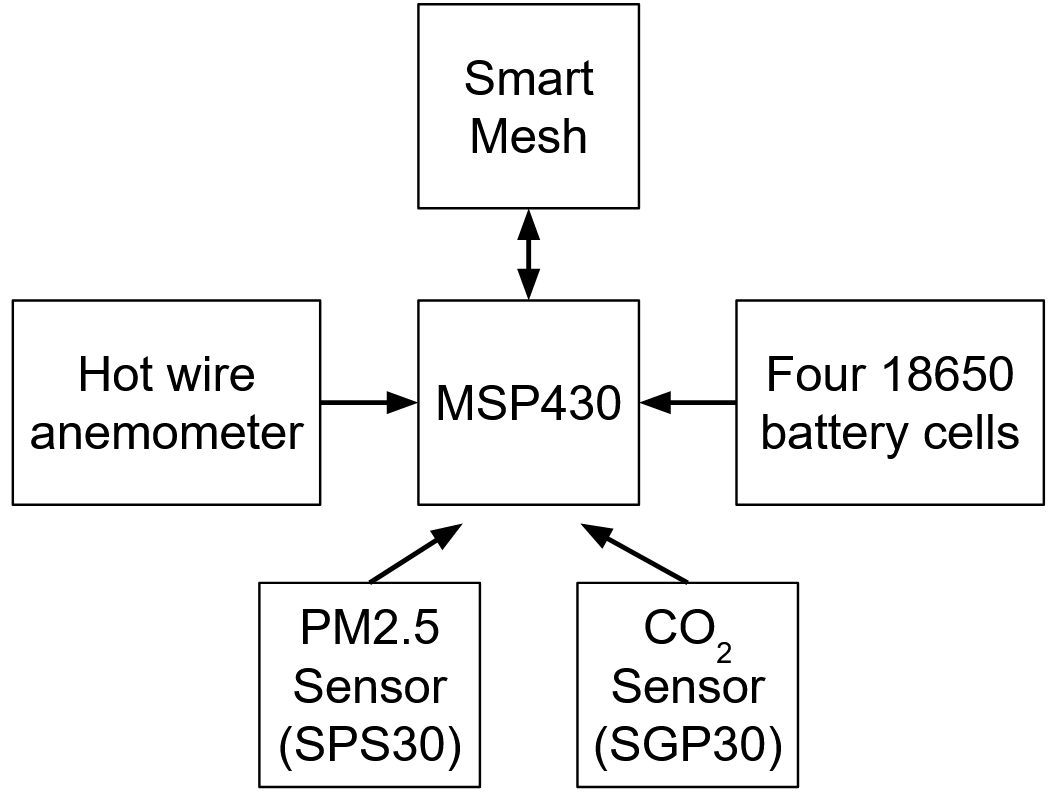
\includegraphics[width=0.8\textwidth]{Pictures/image (5).png}
    \caption[Block Diagram of individual Node]{Block Diagram of individual Node} 
    \label{fig:part1commrin}
\end{figure}

\begin{figure}[H]
    \centering
    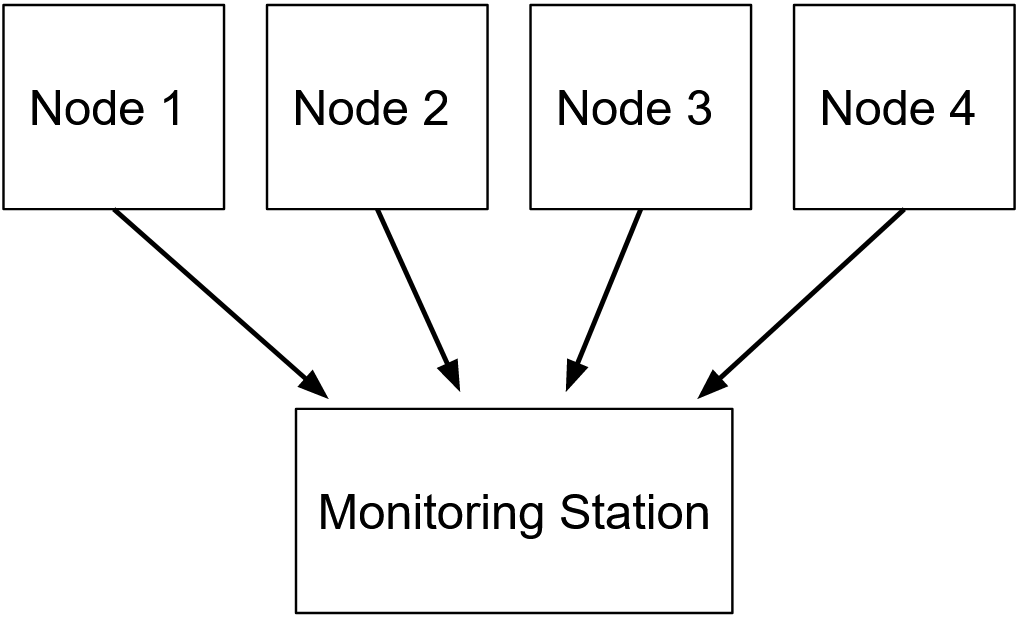
\includegraphics[width=0.8\textwidth]{Pictures/image (6).png}
    \caption[Block Diagram of Meshed System]{Block Diagram of Meshed System} 
    \label{fig:part1commrin}
\end{figure}

\subsection{PCB Design}
\begin{figure}[H]
    \centering
    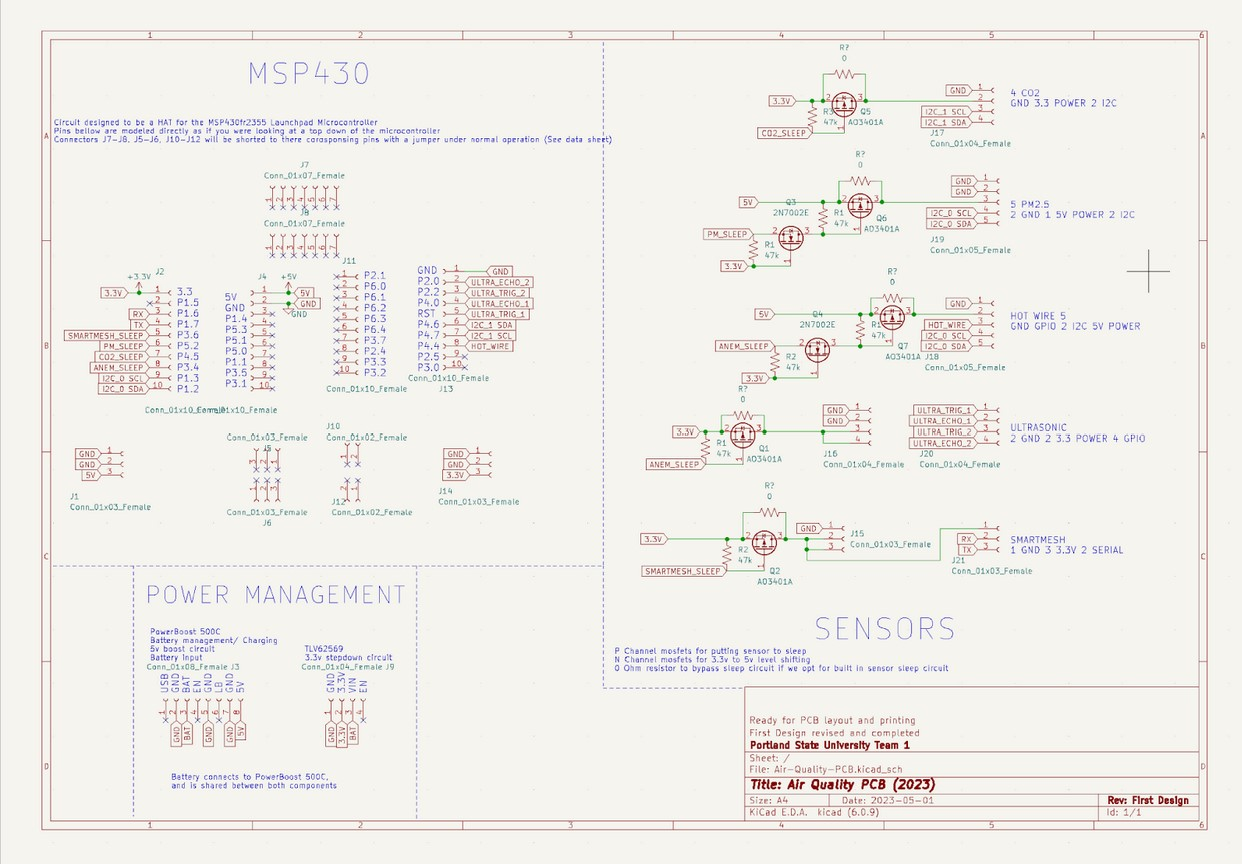
\includegraphics[width=1.0\textwidth]{Pictures/image (8).png}
    \caption[PCB Design]{PCB Design} 
    \label{fig:part1commrin}
\end{figure}

For our PCB, we decided that we wanted our system to be as compact and easy to use as possible. In order to make this a reality we made a hat For the MSP430, or in simpler terms a PCB that is placed directly on top of the MSP430 pins. This was a challenge because we were not able to find standard measurements for the MSP430FR2355 microcontroller, and had to take 15 or so measurements using digital calipers. 

Designing a hat as our board design created unique opportunities that allowed us to streamline and simplify connections, and ended up leading to a cleaner looking final design. We were able to position our power management as close to the microcontoller power ports as possible, and place our signal wires extremely close to where the signals originated from, limiting potential losses that we might have had with longer or messier signal routing.



\subsection{Scheduling}
The team Created a followed the following Gantt charts to reflect the schedule for the project beginning in December of 2022 and concluding in June of 2023.
\begin{figure}[H]
    \centering
    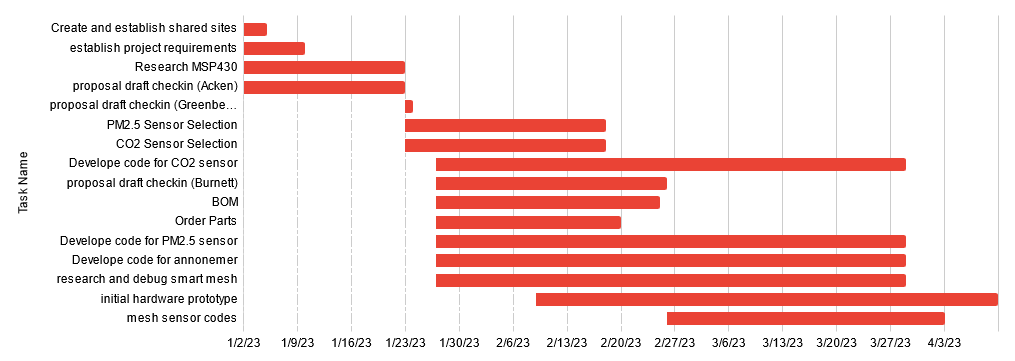
\includegraphics[width=0.8\textwidth]{Pictures/image (3).png}
    \caption[Gantt chart for winter term]{Gantt chart for winter term} 
    \label{fig:part1commrin}
\end{figure}
\begin{figure}[H]
    \centering
    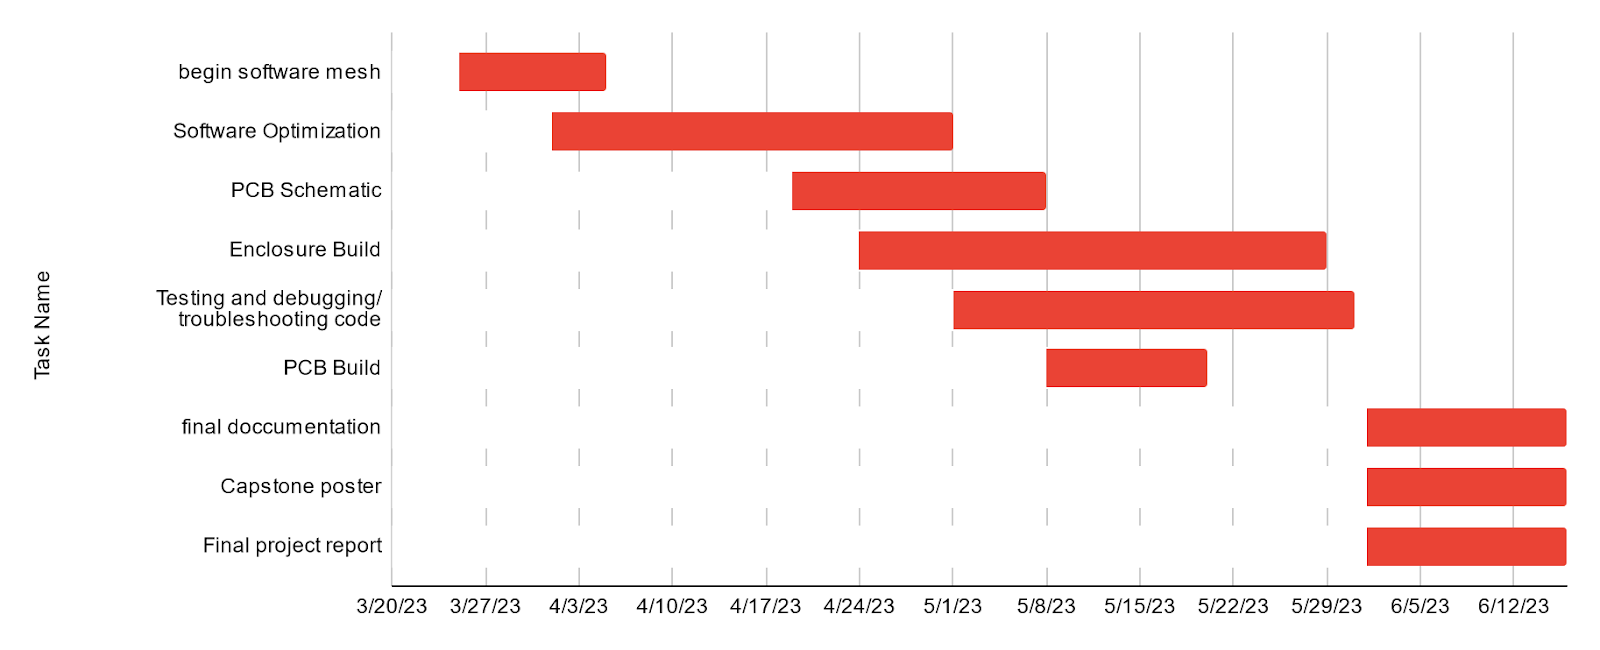
\includegraphics[width=0.8\textwidth]{Pictures/image (4).png}
    \caption[Gantt Chart for spring term]{Gantt Chart for spring term} 
    \label{fig:part1commrin}
\end{figure}